%%%%%%%%%%%%%%%%%%%%%%%%%%%%%%%%%%%%%%%%%%%%%%%%%%%%%%%%%%%%%%%%%%%%%%%%%%%
%
% Template for a LaTex article in Slovak.
%
%%%%%%%%%%%%%%%%%%%%%%%%%%%%%%%%%%%%%%%%%%%%%%%%%%%%%%%%%%%%%%%%%%%%%%%%%%%

\documentclass{article}

\usepackage[utf8]{inputenc}
\usepackage[slovak]{babel}
\usepackage[document]{ragged2e}
\usepackage{amsmath}
\usepackage{siunitx}
\usepackage{multicol}
\usepackage{textcomp}
\usepackage{amsmath, amsthm, amsfonts}
\usepackage{graphicx}
\usepackage{url}
\usepackage{subcaption}
\usepackage{float}
% Theorems
%-----------------------------------------------------------------
\newtheorem{thm}{Theorem}[section]
\newtheorem{cor}[thm]{Corollary}
\newtheorem{lem}[thm]{Lemma}
\newtheorem{prop}[thm]{Proposition}
\theoremstyle{definition}
\newtheorem{defn}[thm]{Definition}
\theoremstyle{remark}
\newtheorem{rem}[thm]{Remark}

% Shortcuts.
% One can define new commands to shorten frequently used
% constructions. As an example, this defines the R and Z used
% for the real and integer numbers.
%-----------------------------------------------------------------
\def\RR{\mathbb{R}}
\def\ZZ{\mathbb{Z}}

% Similarly, one can define commands that take arguments. In this
% example we define a command for the absolute value.
% -----------------------------------------------------------------
\newcommand{\abs}[1]{\left\vert#1\right\vert}

% Operators
% New operators must defined as such to have them typeset
% correctly. As an example we define the Jacobian:
% -----------------------------------------------------------------
\DeclareMathOperator{\Jac}{Jac}

%-----------------------------------------------------------------
\title{Zadanie 3}
\author{Miroslav Kurka\\
  \small Dept. of Biophysics\\
  \small Pavol Jozef Šafárik University in Košice\\
  \small Slovakia 
}

\begin{document}
\maketitle


\section{Úloha}
Majme tyč dĺžky $L = 3,5 m$ pripojenú na potrubie s horúcou kvapalinou. Jedna strana je
pripojená na potrubie a druhá k stene. Vypočítajte rozloženie teploty pozdĺž tyče
v rôznych časoch.
Teplota T sa šíri podľa rovnice vedenia tepla (v 1D v smere osi x):

$$\frac{\partial T}{\partial t} = b \frac{\partial^2 T}{\partial x^2}$$


kde $b = 0,0001 \text{ m}^2\text{s}^{-1}$ je difúzny koeficient. Teplota tyče na začiatku je daná rovnicou:
$$T(t=0,x) = 20\cos\left(\frac{2\pi x}{5}\right)$$

Potom v potrubí začne prúdiť horúca kvapalina a teplota v tyči začne stúpať.
Predpokladáme že teplota horúceho konca tyče v $x = 0$ stúpa s časom $t$ podľa rovnice:

$$T(t,x=0) = 30 \tanh(0,005t) + 20$$
Teplota na konci tyče v $x = L$ (pri stene) ostáva stále rovnaká $T_s = 20C$.

Na numerické riešenie použite explicitnú FTCS metódu pre hodnoty $\alpha = 0,2; 0,5 a 1$.
Pre jednotlivé prípady okomentujte stabilitu numerického riešenia. Vykreslite
rozdelenie teploty pozdĺž tyče pre 5 reprezentatívnych hodnôt času $t \in [0, 2000]$


\subsection{Teória}\label{sec:nothing}
Úloha je založená na riešení diferenciálnej rovnice pomocou FTCS metódy. Táto využíva doprednú časovú a centrálnu priestorovú diferenciu pre aproximáciu prislušných derivácií (viz. Obr. \ref{diskretizacia})\cite{Zukovic}. 
\begin{figure}
    \centering
    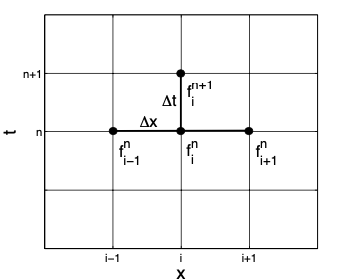
\includegraphics[width=1\textwidth]{ftcs.png}
    \caption{Diskretizačná schéma pre FTCS metódu (Prevzaté z \cite{Zukovic})}
    \label{diskretizacia}
\end{figure}


\begin{equation}
    \frac{\partial T}{\partial t} = b \frac{\partial^2 T}{\partial x^2}
\end{equation}
podľa diskretizačnej schémy \ref{diskretizacia} možeme prepísať ako:
\begin{equation}
\frac{T_{i,j+1}-T_{i,j}}{dt} = b \frac{T_{i+1,j}-2T_{i,j}+T_{i-1,j}}{dx^2}
\end{equation}
Následne si vyjadríme $T_{i,j+1}$:
\begin{equation}
    T_{i,j+1} = T_{i,j} + \alpha (T_{i+1,j} - 2T_{i,j} + T_{i-1,j})
\end{equation}
kde $\alpha = \frac{b dt}{dx^2}$. 


Pre FCTS metódu platí $\Delta t  \leq  \frac{\Delta x^2 }{2\alpha}$ tzv. podmienka stability. Ak táto podmienka nie je splnená metóda sa stane nestabilnou.\cite{wiki}

\subsection{Výsledky}
Na Obr.\ref{fig:ftcs} sú zobrazene riešenia pre rôzne hodnoty alfa. Na grafoch je zobrazená teplota v čase pre rôzne body tyče. Farebne sú zobrazené rôzne časy $t$ z intervalu $[0,2000]$. Tie sú konkrétne 0, 500, 1000, 1500 a 2000 podľa zadania. Časový krok je $dt = \frac{dx^2}{2\alpha}$ a priestorový krok je $dx = 0.1$ pre všetky tri grafy. Na vytvorenie grafov bolo nutné použiť knižnicu qtplot, pretoze octave základná knižnica nevie vykreslovať tak vysoké hodnoty float hodnôt aké sú pre $\alpha = 1$.
\begin{figure}[H]
    \centering
    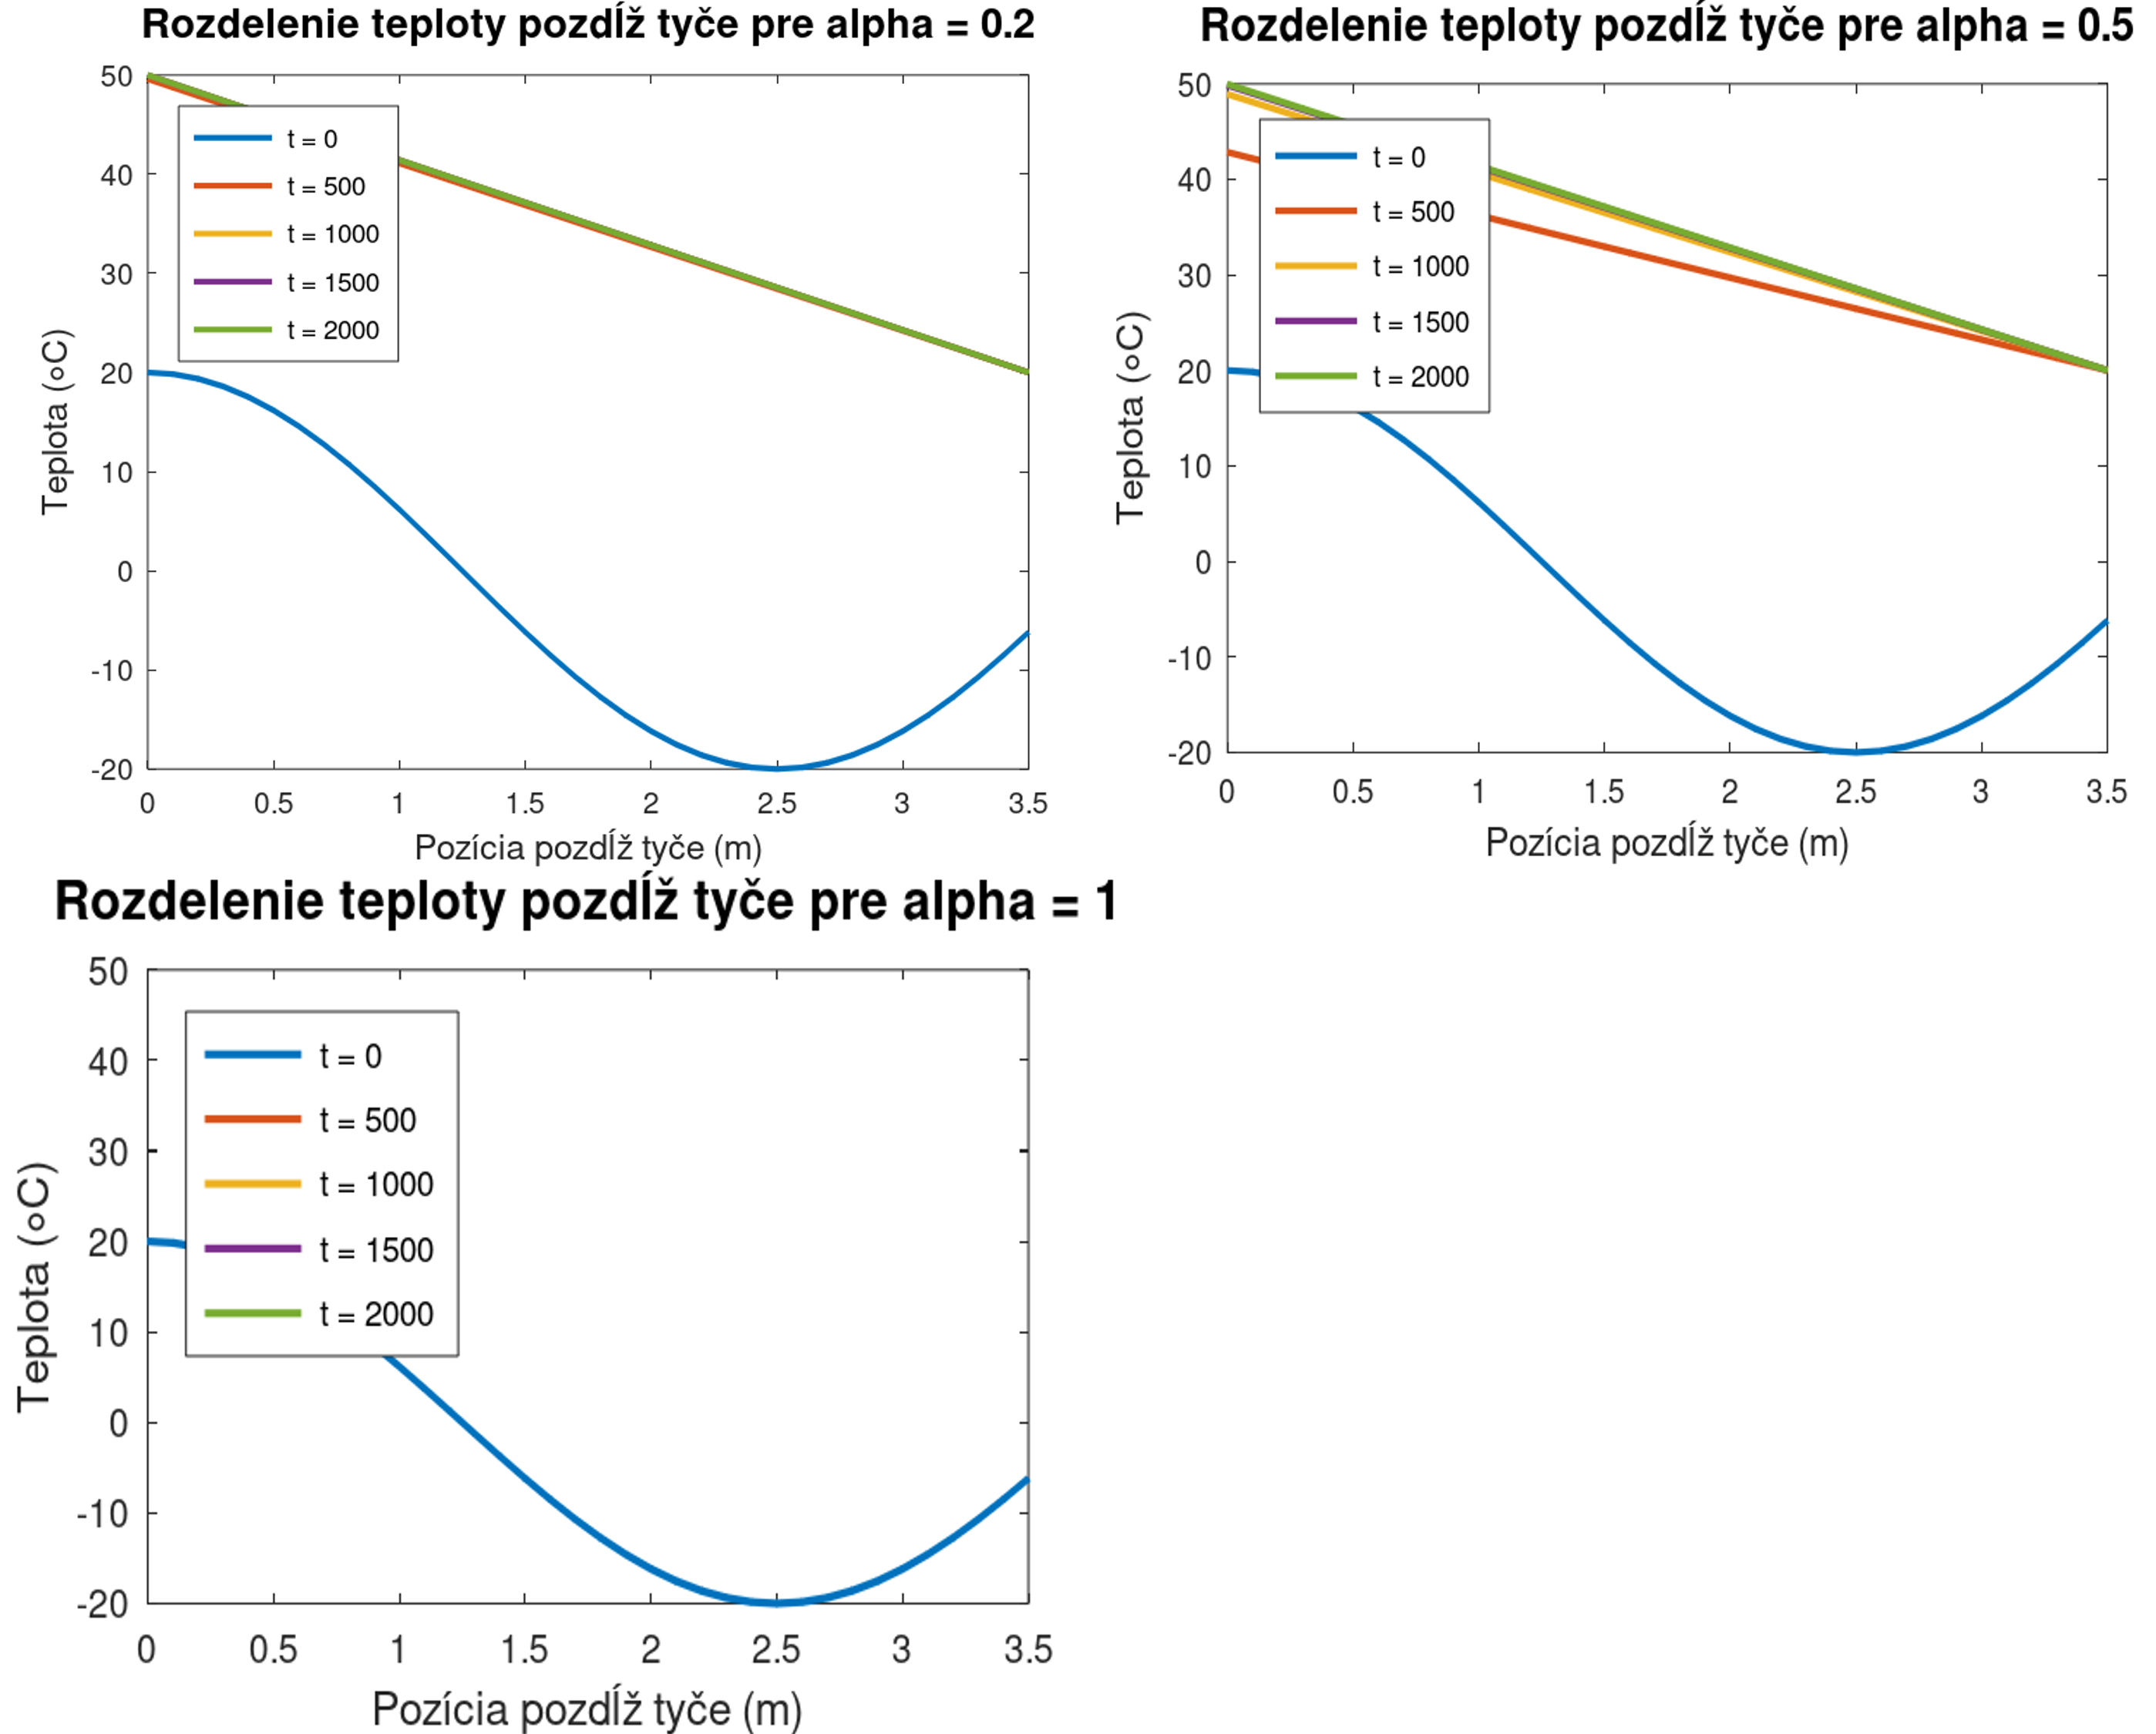
\includegraphics[width=1\textwidth]{hw3pic_correct.png}
    \caption{Riešenia pre rôzne hodnoty $\alpha$}
    \label{fig:ftcs}
\end{figure}



\pagebreak

\subsection{Záver a Diskusia}
Z grafov na Obr. \ref{fig:ftcs} je zrejmé, že pre $\alpha = 0.2$ a $\alpha = 0.5$ sú riešenia stabilné. Pre $\alpha = 1$ je riešenie nestabilné. 
\bibliographystyle{alpha}
% Bibliography
%----------------------------------------------------------
\begin{thebibliography}{99}

\bibitem{Zukovic}Žukovič, M. (2015) \emph{Počítačová fyzika I} Dostupné z \url{https://ufv.science.upjs.sk/zukovic/download/POF1/Literatura/Pocitacova%20fyzika%20I.pdf}
\bibitem{wiki} Wikipedia (2019) \emph{Forward Time Centered Space method} Dostupné z \url{https://en.wikipedia.org/wiki/FTCS_scheme}
\end{thebibliography}

\end{document}
